% version 1.00, date 12/05/16, auteur(s) Pierre Porche, Sergi Colomies
\documentclass[compress,xcolor=dvipsnames]{beamer}

%Pour les schémas d'architecture
\usepackage{etex}
\usepackage{tikz}
\usetikzlibrary{shapes,arrows,chains,backgrounds,fit}
%FIN Pour les shémas d'architecture

\usepackage[french]{babel}
\selectlanguage{french}
\usepackage[utf8]{inputenc}
\usepackage[T1]{fontenc}
\usepackage{tikz}
\usepackage{hhline}
\usepackage{wrapfig}
\usepackage{multirow}
\usepackage{multicol}
%\usepackage{pgf-pie}
\usepackage{pgfplots}
\usepackage{pdfpages}
\usepackage{vocabulaireUnipikPresentation}
\usepackage{commun/vocabulaireCommun}
\usepackage{hyperref}
\usepackage{movie15}
\usepackage{xcolor}
\usepackage{lscape}
\usepackage{booktabs}
\usepackage{multirow}
\usepackage{colortbl}
\usepackage{longtable}
\usepackage{color}

\newcommand{\tabincell}[2]{\begin{tabular}{@{}#1@{}}#2\end{tabular}}

\usetheme{eastpic}%{Berlin}%{Madrid}

 
 
%Information to be included in the title page:
\title{Revue de PIC}
\date{\today}
\author{Unipik}
\institute{\insa}

\setbeameroption{show notes}

 
\begin{document}

\speaker{\Pierre} 

\begin{frame}[plain]
	\titlepage
\end{frame}

\begin{frame}{Sommaire}
	\tableofcontents%[hideallsubsections]
\end{frame}
 
\section[Présentation]{Présentation}
\subsection{} % PAs besoin de titre

\begin{frame}
\frametitle{Présentation de l'équipe}
	\begin{figure}
		\includegraphics[scale=0.25]{images/organigrammeFonctionnel.png}
		\caption{Organigramme fonctionnel}
		\label{OF}
	\end{figure}
\end{frame}

\speaker{Mélissa Bignoux}
\begin{frame}
\frametitle{Présentation du client}
	\begin{center}
		UNICEF
	\end{center}
	\begin{itemize}
		\item Un des principaux organismes d’aide humanitaire et de développement
		\item Acteur partout dans le monde en faveur des droits de chaque enfant
	\end{itemize}
	
	\begin{center}
		UNICEF Seine-Maritime
	\end{center}
	Ses actions principales sont : 
	\begin{itemize}
		\item La sensibilisation aux droits de l'enfant
		\item Les événements 
		\item Les ventes sur stands
	\end{itemize}
	
\end{frame}
\speaker{Mélissa Bignoux}
\begin{frame}
\frametitle{Présentation du sujet}
Outil de gestion informatique des interventions externes suivantes :

	\begin{itemize}
		\item Les plaidoyers dans les \'ecoles
		\item Les actions frimousses
		\item Les projets de lycéens et d'étudiants
		\item Les actions ponctuelles
	\end{itemize}
	
\end{frame}

\section[Déroulement du projet]{Déroulement du projet}
% version 1.00, date 08/01/17, auteur Florian Leriche
\speaker{\Kafui}

\begin{frame}

\frametitle{Mise en place du \SMQ}
	\begin{block}{Travail effectué}
		\begin{itemize}
			\item Rédaction d'artefact afin de centraliser les règles à suivre (\PQ{},\PGC{});		
			\item Identification de risques et opportunités afin de contrôler ceux-ci (suivi assuré grâce au \PRO);
			\item Mise en place d'indicateurs concernant divers aspects du projet (gestion de projet, satisfaction client. qualité du développement).
		\end{itemize}      
	\end{block}
\end{frame}


% version 1.00, date 08/01/17, auteur Florian Leriche
\speaker{\Julie}
\subsection{} % PAs besoin de titre

\begin{frame}
\frametitle{ }
	\begin{block}{ }
		\begin{itemize}
			\item 
		\end{itemize}      
	\end{block}
\end{frame}

\subsection*{Lot 1}
\input{sources/lots/04_lot1.tex}

\subsection*{Lot 2}
\speaker{\Florian}

\begin{frame}
\frametitle{Lot 2}
\begin{block}{Fonctionnalités du lot 2}
	\begin{itemize}
		\item Ajout, modification et suppression d'un bénévole
		\item Ajout, modification et suppression d'un établissement
		\item Mailing
		\item Formulaire de demande
		\item Aide à l'affectation d'une intervention à un bénévole
		\item Attribution et mise à jour d'une intervention par un bénévole
		\item Mails de rappel à l'établissement et au bénévole
	\end{itemize}
\end{block}
\end{frame}

\begin{frame}
\frametitle{Lot 2}
\begin{block}{Difficultés rencontrés}
	\begin{itemize}
		\item hébergement ?
		\item la BD ?
		\item pas de smtp pour le mailing ?
		\item Sinon aucune niveau dev
	\end{itemize}
\end{block}
\end{frame}

\begin{frame}
\frametitle{Lot 2}
\begin{block}{Solutions}
	\begin{itemize}
		\item Franchement aucune idées
	\end{itemize}
\end{block}
\end{frame}

\begin{frame}
\frametitle{Lot 2}
\begin{block}{En quoi c dla qualité ??? c une opportunité ?}
	\begin{itemize}
		\item Digital Ocean
	\end{itemize}
\end{block}
\end{frame}

\subsection*{Lot 3}
\speaker{\Francois}

\begin{frame}
	\frametitle{Lot 3}
	\begin{block}{Risques et opportunités}
		\begin{itemize}
			\item Opportunité d'hébergement chez Quantic déclenchée
			\item Risque d'absence de serveur cloturé
			\item Rattrapage du retard grâce à la renégociation du cahier des charges
		\end{itemize}
	\end{block}
	\begin{block}{Fonctionnalités du lot 3}
		\begin{itemize}
			\item Gestion des frimousses
			\item Géolocalisation
		\end{itemize}
	\end{block}
\end{frame}

\begin{frame}
	\frametitle{Lot 3}
	\begin{block}{Géolocalisation}
		\begin{itemize}
			\item Attributs des entités Bénévole et Établissement
			\item Filtres par lieu
			\item Mailing par lieu
			\item Cartes pour visualiser les listes
		\end{itemize}
	\end{block}
\end{frame}

\begin{frame}
	\frametitle{Lot 4}
	\begin{block}{Fonctionnalités du lot 4}
		\begin{itemize}
			\item Utilisation de Google Chart pour la gestion des statistiques 
			\begin{itemize}
				\item Sur le nombre d'interventions
				\item Sur les ventes et les dons
			\end{itemize}
		\end{itemize} 
	\end{block}
\end{frame}

\subsection*{Lot 4}
% version 1.00, date 30/11/16, auteur Kafui Atanley

%La fonctionnalité 11 concerne le module de statistiques concernant les données de l’Uni-
%cef. Ce module de statistiques contribuera à effectuer le bilan annuel. Il devra permettre de
%comptabiliser le nombre d’établissement partenaires ainsi que leur type. Il devra aussi per-
%mettre de comptabiliser le nombre de personnes ayant été sensibilisé. Il devra permettre de
%comptabiliser le nombre d’intervention effectué, les thèmes les plus plebiscités en fonction
%de critère tel que le type d’établissement, le niveau scolaire des participants. Il devra enfin
%permettre de comptabiliser les ventes effectuées à l’année en fonction de la zone géogra-
%phique et du chiffre d’affaire. Il devra être possible de générer un rapport au format PDF ou
%au format CSV figurant chacune de ces données pour l’année actuelle. L’équipe Projet INSA
%Certifié devra être force de proposition compte à la représentation graphique de celle-ci de
%celle-ci.

\section{Lot 4}
\subsection{Fonctionnalité 11}

La fonctionnalité 11 consistera à mettre en place un module de statistique. Ce module de statistique étant utilisé pour établir une bilan de fin d'année, il devra être le plus précis possible.
Ce module de statistique devra porter sur la gestion des interventions et des ventes associées.
Une attention particulière sera porté sur la gestion des devises.
Il devra être possible de :
\begin{itemize}
\item comptabiliser les interventions de type action éducative par thème, type d'établissement, nombre de participant;
\item comptabiliser les interventions de type frimousse par type d'établissement, nombre de participant, chiffre d'affaire engrangé;
\item comptabiliser les ventes par chiffre d'affaire.
\end{itemize}
Ces données devront pouvoir être générées par année. La représentation graphique de ces données devra être faite à l'aide de diagramme circulaire et/ou de diagramme en barre. La maquette \ref{fonctionnalite11Stat} présente comment sera figurée la liste des ventes. La repésentation graphique pourra également être figurée de manière alternative selon le temps restant en PIC.
Il devra être possible d'avoir des tableaux représentant ces données. Ces tableaux devront pouvoir être exportés au format CSV et PDF.

\begin{figure}[H]
	\centering
	\includegraphics[scale=0.4]{images/maquettes/fonctionnalite11Stat.png}
	 \caption{Maquette~: Maquette du module de statistiques}
	 \label{fonctionnalite11Stat}
\end{figure}



% version 1.00, date 08/01/17, auteur Florian Leriche
\speaker{\Juliana}
\subsection{} % PAs besoin de titre

\begin{frame}
\frametitle{ }
	\begin{block}{ }
		\begin{itemize}
			\item 
		\end{itemize}      
	\end{block}
\end{frame}

\section[Gestion de projet]{Gestion de projet}
% version 1.00, date 08/01/17, auteur Florian Leriche
\speaker{\Pierre}
\subsection{} % PAs besoin de titre

\begin{frame}
\frametitle{Relation client au sein du PIC}
	\begin{block}{La relation client}
		\begin{itemize}
			\item Implication forte du client ;
			\item Réunions fréquentes.
		\end{itemize}      
	\end{block}
	\begin{block}{Révision du cahier des charges initial}
		\begin{itemize}
			\item Attentes réelles différentes des attentes écrites ;
			\item Changements en cours de projet ;
			\item Contexte client inédit pour l'équipe PIC.
		\end{itemize}      
	\end{block}
\end{frame}


\begin{frame}
\frametitle{La gestion des ressources du PIC UNICEF}
	\begin{block}{Outils pour la gestion des ressources}
		\begin{itemize}
			\item Diagramme de GANTT ;
			\item Scrum Board.
		\end{itemize}      
	\end{block}
\end{frame}


\begin{frame}
\frametitle{Scrum Board}
	\begin{figure}
		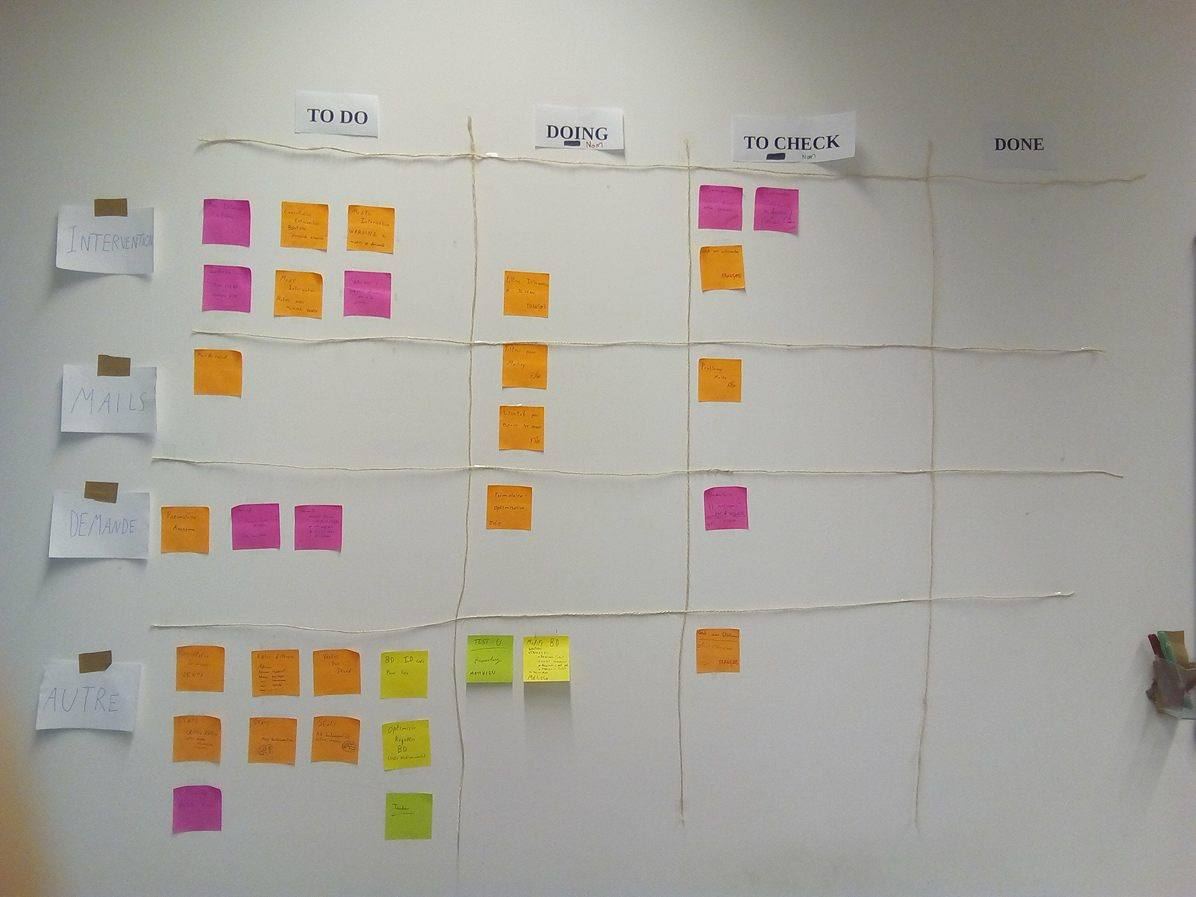
\includegraphics[scale=0.2]{images/kanban.jpg}
		\caption{Notre Scrum Board}
		\label{Kn}
	\end{figure}
\end{frame}
	

\begin{frame}
\frametitle{Retour sur la gestion de projet}
	\begin{block}{Une nouvelle expérience}
		\begin{itemize}
			\item Découverte de la gestion de projet ;
			\item Acquisition de compétences d'ingénieur ;
			\item Dernière livraison le 14 décembre 2016.
		\end{itemize}      
	\end{block}
\end{frame}

\section[Retour d'expérience]{Retour d'expérience}
% version 1.00, date 08/01/17, auteur Florian Leriche
\speaker{\Kafui}
\subsection{} % PAs besoin de titre

\begin{frame}

\frametitle{Retour d'expérience sur la démarche Qualité}
	\begin{block}{Bilan}
		\begin{itemize}
			\item qualitayFacilo		
			\item qualitayFacilo
			\item qualitayFacilo
		\end{itemize}      
	\end{block}
\end{frame}

\begin{frame}

\frametitle{Retour d'expérience sur la démarche Qualité}
	\begin{block}{Ressenti de l'équipe}
		Avantages : 
		\begin{itemize}
			\item qualitayFacilo	
			\item qualitayFacilo
			\item qualitayFacilo
		\end{itemize}   
		Inconvénients :
		\begin{itemize}
			\item qualitayFacilo	
			\item qualitayFacilo
			\item qualitayFacilo			
		\end{itemize}   
	\end{block}
\end{frame}


\section[Conclusion]{Conclusion}
% version 1.00, date 08/01/17, auteur Florian Leriche
\speaker{\Pierre}
\subsection*{} % PAs besoin de titre

\begin{frame}
\frametitle{Conclusion}
	\begin{block}{Le PIC UNICEF}
		\begin{itemize}
			\item Une équipe soudée et volontaire ;
			\item Un apprentissage en condition réelles ;
			\item Un client proche du projet ;
			\item Un projet réussi.
		\end{itemize}      
	\end{block}
\end{frame}

\speaker{}
\begin{frame}
	\frametitle{Merci de votre attention !}
	\begin{center}\color{black}
		\Huge{Des questions ?}
	\end{center}
\end{frame}


\end{document}

